\chapter{Présentation du cadre du projet}



\newpage
 
 
\section{Introduction}
Ce premier chapitre comportera plusieurs parties dont on peut citer l’organisme d’accueil, la 
problématique du projet, la solution proposée ainsi que notre méthodologie adoptée pour le développement de ce projet.

\section{Présentation de l'organisme d'accueil}
Notre projet se déroule au sein de l’entreprise UNIBRO Distribution, une société spécialisée dans la distribution de produits alimentaires et de grande consommation. Elle se distingue par son organisation logistique, son professionnalisme et sa capacité à répondre efficacement aux besoins du marché. UNIBRO Distribution s’engage à assurer un service fiable, basé sur la qualité, la rapidité et la satisfaction de ses partenaires commerciaux.\cite{ref1}
\begin{figure}[H]
  \centering
    
\includegraphics[scale=0.3]{images/general/logo_unibro-removebg-preview}
  \caption{Logo de la société UNIBRO Distribution}
\end{figure}
\subsection{Domaines d’activités}
UNIBRO Distribution se spécialise dans les domaines suivants :
\begin{itemize}[label=$\rightarrow$]
\item 
 Distribution de produits : Approvisionnement et distribution de produits alimentaires et de grande consommation.
\item 
 Logistique : Gestion du transport, du stockage et de la livraison des marchandises.
\item 
 Gestion commerciale : Relations avec les fournisseurs et les clients, suivi des commandes et des ventes.
\item Service client : Satisfaction des partenaires commerciaux et respect des délais de livraison.
\end{itemize}

\section{Contexte du projet}
Dans cette partie, nous décrivons l'étude de l'existant, les limites ainsi que la solution proposée.
\subsection{Etude de l'existant}
Cette section présente une analyse du système existant de gestion du pointage et des procédures RH, en mettant en évidence ses principales caractéristiques ainsi que ses limites. 
\subsubsection{Description de l'existant}
Le système actuel de gestion du pointage et des procédures RH repose sur des méthodes traditionnelles :
\begin{itemize}
\item Les registres manuels (feuilles de présence) : Les employés signent un document papier à l’arrivée et au départ.

\item  Les systèmes à badges (RFID/Magnétiques) : L’identification repose sur la possession d’une carte que l’employé passe devant un lecteur.

\item L’authentification par codes (PIN) : L’employé saisit un code personnel sur un clavier numérique.
\item Justification d’absence physique : Les justificatifs sont remis manuellement sans dépôt ni archivage numérique.
\item Gestion traditionnelle des primes : L’attribution et le suivi des primes sont effectués manuellement sans consultation numérique pour les employés.
\item Absence de consultation du salaire mensuel : Les employés ne peuvent pas vérifier le statut de leur salaire du mois en cours.

\end{itemize}


\subsubsection{Critique de l'existant et problématique}
Nous citons ci-dessous quelques problèmes liés au système existant :
%===========utiliser une liste à puces simple 
\begin{itemize}
 \item  Erreur humaine : saisie manuelle sujette à des oublis ou des erreurs.

\item Fraude : possibilité de pointage pour un autre employé.

\item Pas de suivi en temps réel : impossibilité de visualiser immédiatement la présence ou l’absence.

\item Gestion lourde : centralisation et analyse des données complexes et fastidieuses..
\item Procédures administratives lentes dues à l’utilisation de documents papier. 
\item Manque de transparence pour les employés concernant les congés, absences, primes et salaires. 
\item Risque de perte ou de détérioration des documents physiques.
\end{itemize}

\subsection{Solution proposée}
Afin de résoudre le problème mentionné plus haut lors de ce projet de fin d'études,
nous allons nous concentrer sur la réalisation d'un logiciel intelligent de gestion des ressources humaines de pointage automatique avec reconnaissance faciale.
Cela aidera à créer un emplacement centralisé pour organiser toute information relative à la gestion des données de présence de nos employés.
Les employés du département de gestion des ressources humaines auront l'opportunité de recevoir des rapports détaillés en peu de temps, parmi lesquels ils seront capables de suivre l'indicateur de présence, de retard ou d'absence des employés.
Le processus comprend les éléments suivants :
\begin{enumerate}
    \item  Collecte de données : prise en charge de la photo du visage des employés avec caméra.
\item   Intégration et traitement des données : enregistrement automatique de la présence des employés avec indication de leur heures d'entrée et de sortie.
\item  Traitement et analyse des données : visualisation et suivi des statistiques avec l'aide d'une interface intuitive de tableau de bord.
\end{enumerate}
À l'aide de ce système d'information, l'entreprise aura une occasion d'optimiser la gestion de son personnel et de supprimer les erreurs dans le processus de pointage des employés.

\section{Méthodologie de travail}

Pour assurer une bonne gestion de notre projet, il est nécessaire de sélectionner une métho-
dologie de travail appropriée. Au sein du domaine du développement logiciel, il y a diverses
méthodologies de travail qui existent, notamment les méthodologies traditionnelles et les mé-
thodologies Agile. Les méthodologies Agile ont été mises en place pour combler certains faibles
des méthodologies traditionnelles. Il est à noter que les méthodologies Agile mettent l’em-
phase sur le travail en équipe, l’adaptabilité et la réalisation continue de produits fonctionnels
au cours du développement du projet. Parmi les méthodologies Agile qui sont familières, il y a
le Scrum, Kanban et Extreme Programming (XP). Les méthodologies Agile sont basées sur un
cycle de développement court appelé itération.

Pour la réalisation de notre projet de développement d'un système de gestion des ressources
humaines et de pointage automatique, nous avons décidé d'utiliser le cadre de travail Scrum.
La raison qui motive ce choix est qu'il est nécessaire de faire rapidement les ajustements
nécessaires dans le système en fonction des nouvelles exigences des utilisateurs. Scrum est un
cadre de travail simple qui permet aux individus, groupes et aux organisations de créer de la
valeur par des solutions adaptatives pour résoudre des problèmes complexes \cite{Scrum}. \newline
La philosophie
de Scrum est la possibilité d'orienter le projet en cours en fonction des besoins.
Le cadre de travail Scrum utilise le découpage du projet par des itérations dénommées
sprints. Le sprint est une itération limitée dans le temps à un mois ou moins, lors de laquelle
l'équipe travaille avec une liste spécifique de fonctionnalités fournissant de la valeur au produit.
Scrum ne fournit aucune information sur le processus de spécification, programmation et
test de produit. Cependant, il comprend un certain nombre d'éléments, notamment :

\begin{itemize}[label=$\bullet$]
\item des rôles spécifiques ;
\item des événements ;
\item des artéfacts ;
\item des règles de fonctionnement.
\end{itemize}

La figure 2 présente une vue globale du fonctionnement de la méthodologie Scrum [B2].

\begin{figure}[H]
  \centering
    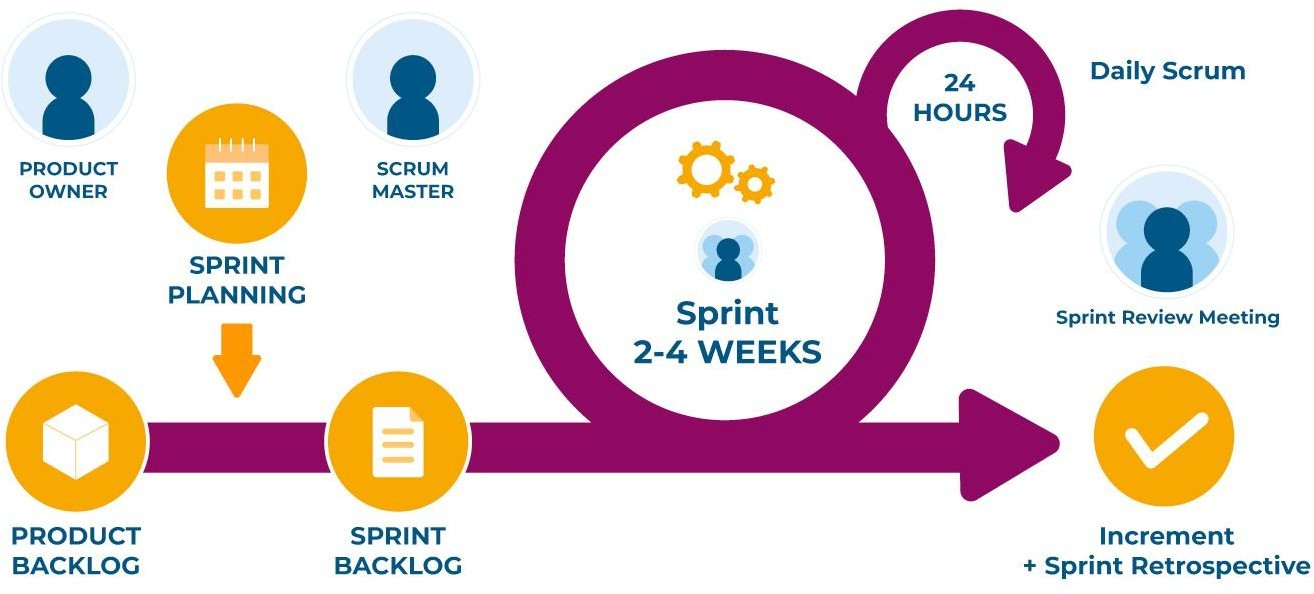
\includegraphics[scale=0.3]{images/general/scrum.png}
  \caption{Cycle de vie d’un projet avec la méthodologie de Scrum Agile}
\end{figure}




 
\section{Conclusion}

Ce chapitre constitue une étape primordiale pour fixer les repères de notre projet durant lequel nous avons présenté l’organisme d’accueil et dégagé des attentes du projet après avoir étudié et critiqué l’existant. À la fin, nous avons présenté la méthodologie de travail à utiliser.
 








